\documentclass[../thesis.tex]{subfiles}

\begin{document}

\appendix

\chapter{Data Description}
\label{chap:data_desc}

\noindent In this appendix we present a descriptive overview of the data used in this thesis. This includes: an overview and explanation of the variables used (\ref{sec:variables}), the \texttt{R}-packages (\ref{sec:r_pack}) used and some relevant plots (\ref{sec:rel_plots}) to support the finding in the thesis. The source code used to produce the relevant plots can be found in appendix (\ref{chap:souce_code}).  

\section{Variables}
\label{sec:variables}

\section{\texttt{R}-packages}
\label{sec:r_pack}

\section{Descriptive Statistics}
\label{sec:desc_stat}


\begin{scriptsize}
\begin{tabularx}{\textwidth}{P{3cm}RRRRRRRRRR}
\caption{Patient characteristics: HFpEF variables}\label{tab:desc_stat_HFpEF_variables}\\
\toprule
\textbf{Variable} & $n$ & \# Na & Min & Max & $\bar{x}$ & $\widetilde{x}$ & $s$ & $q_1$ & $q_3$ \\ 
\midrule
\endfirsthead
\caption*{\textbf{Table \ref{tab:desc_stat_HFpEF_variables}:} Patient characteristics: HFpEF variables (\textit{continued})}\\
\toprule
 \textbf{Variable} & $n$ & \# Na & Min & Max & $\bar{x}$ & $\widetilde{x}$ & $s$ & $q_1$ & $q_3$ \\ 
\midrule
\endhead
\multicolumn{10}{c}{PANEL I: Identification}\\
\midrule
  patientid & 193 &   0 &   3.0 &   246.0 &  120.6 &  115.0 &   70.5 &  60.0 &  182.0 \\ 
\midrule
\multicolumn{10}{c}{PANEL II: Demographics}\\
\midrule
  age & 193 &   0 &  29.0 &   100.8 &   76.3 &   78.9 &   12.1 &  69.5 &   85.4 \\ 
  gender & 193 &   0 &   0.0 &     1.0 &    0.6 &    1.0 &    0.5 &   0.0 &    1.0 \\ 
  white & 193 &   0 &   0.0 &     1.0 &    0.7 &    1.0 &    0.5 &   0.0 &    1.0 \\ 
  asian & 193 &   0 &   0.0 &     1.0 &    0.1 &    0.0 &    0.2 &   0.0 &    0.0 \\ 
  black & 193 &   0 &   0.0 &     1.0 &    0.3 &    0.0 &    0.4 &   0.0 &    1.0 \\ 
  otherethnicity & 193 &   0 &   0.0 &     1.0 &    0.0 &    0.0 &    0.1 &   0.0 &    0.0 \\ 
\multicolumn{10}{c}{PANEL III: Admission symptoms}\\
\midrule
  breathless & 185 &   8 &   0.0 &     1.0 &    0.8 &    1.0 &    0.4 &   1.0 &    1.0 \\ 
  chestpain & 186 &   7 &   0.0 &     1.0 &    0.0 &    0.0 &    0.2 &   0.0 &    0.0 \\ 
  orthopnoea & 184 &   9 &   0.0 &     1.0 &    0.3 &    0.0 &    0.5 &   0.0 &    1.0 \\ 
  peripheraloedema & 185 &   8 &   0.0 &     1.0 &    0.5 &    0.0 &    0.5 &   0.0 &    1.0 \\ 
  palpdizzyfalls & 184 &   9 &   0.0 &     1.0 &    0.2 &    0.0 &    0.4 &   0.0 &    0.0 \\ 
  pnd & 184 &   9 &   0.0 &     1.0 &    0.3 &    0.0 &    0.4 &   0.0 &    1.0 \\ 
\midrule
\multicolumn{10}{c}{PANEL IV: Admission signs}\\
\midrule
  sbp & 184 &   9 &   0.0 &   242.0 &  145.3 &  145.0 &   35.0 & 125.0 &  167.0 \\ 
  dbp & 184 &   9 &   0.0 &   195.0 &   80.0 &   80.0 &   22.9 &  66.8 &   89.0 \\ 
  map & 188 &   5 &   0.0 &   182.0 &   99.6 &  100.2 &   26.1 &  85.3 &  112.4 \\ 
  admissionwgt & 190 &   3 &   0.0 &   158.0 &   66.4 &   72.2 &   35.9 &  52.8 &   89.0 \\ 
  height & 190 &   3 &   0.0 &   185.0 &  121.8 &  158.0 &   70.6 & 110.1 &  166.0 \\ 
  bmiadmission & 191 &   2 &   0.0 &   107.1 &   23.8 &   25.9 &   15.8 &  18.2 &   33.4 \\ 
  weightchange & 170 &  23 & -22.0 &    42.3 &   -0.1 &    0.0 &    5.5 &   0.0 &    0.0 \\ 
  admissionsbnp & 184 &   9 &   0.0 &   135.0 &    3.4 &    1.0 &   15.7 &   1.0 &    2.0 \\ 
  pulse & 184 &   9 &   0.0 &   211.0 &   83.8 &   83.0 &   23.7 &  69.8 &   95.0 \\ 
  bp & 192 &   1 &   0.0 &     1.0 &    0.8 &    1.0 &    0.4 &   1.0 &    1.0 \\ 
  asympthf & 186 &   7 &   0.0 &     1.0 &    0.1 &    0.0 &    0.3 &   0.0 &    0.0 \\ 
  devicetherapy & 164 &  29 &   0.0 &     1.0 &    0.0 &    0.0 &    0.1 &   0.0 &    0.0 \\ 
\midrule
\multicolumn{10}{c}{PANEL V: Risk factors}\\
\midrule
  a-fib & 189 &   4 &   0.0 &     1.0 &    0.5 &    0.0 &    0.5 &   0.0 &    1.0 \\ 
  copdasthma & 190 &   3 &   0.0 &     1.0 &    0.4 &    0.0 &    0.5 &   0.0 &    1.0 \\ 
  irondef &  69 & 124 &   0.0 &     1.0 &    0.6 &    1.0 &    0.5 &   0.0 &    1.0 \\ 
  obesity & 185 &   8 &   0.0 &     1.0 &    0.5 &    1.0 &    0.5 &   0.0 &    1.0 \\ 
  obesitybmi30 &  72 & 121 &   1.0 &     1.0 &    1.0 &    1.0 &    0.0 &   1.0 &    1.0 \\ 
  nyhaclass & 187 &   6 &   0.0 &     4.0 &    3.1 &    4.0 &    1.3 &   1.5 &    4.0 \\ 
  dm & 188 &   5 &   0.0 &     1.0 &    0.5 &    1.0 &    0.5 &   0.0 &    1.0 \\ 
  ihd & 186 &   7 &   0.0 &     1.0 &    0.4 &    0.0 &    0.5 &   0.0 &    1.0 \\ 
  osa &  22 & 171 &   0.0 &     1.0 &    0.9 &    1.0 &    0.3 &   1.0 &    1.0 \\ 
\midrule
\multicolumn{10}{c}{PANEL VI: Comorbidities}\\
\midrule
  comorbidities & 193 &   0 &   0.0 &     9.0 &    4.2 &    4.0 &    1.8 &   3.0 &    5.0 \\ 
\midrule
\multicolumn{10}{c}{PANEL VII: Electrocardiography}\\
\midrule
  ecgblock & 171 &  22 &   0.0 &     1.0 &    0.3 &    0.0 &    0.4 &   0.0 &    1.0 \\ 
  ecgblockcomment & 187 &   6 &   0.0 &     1.0 &    0.3 &    0.0 &    0.5 &   0.0 &    1.0 \\ 
  ecgqrsduration & 157 &  36 &  55.0 &   177.0 &  101.3 &   98.0 &   20.8 &  88.0 &  112.0 \\ 
  ecgqrsother & 193 &   0 &   0.0 &     1.0 &    0.0 &    0.0 &    0.2 &   0.0 &    0.0 \\ 
  ecgrate & 159 &  34 &  41.0 &   191.0 &   83.0 &   80.0 &   23.1 &  70.0 &   92.0 \\ 
  ecgrhythmother & 193 &   0 &   0.0 &     1.0 &    0.1 &    0.0 &    0.2 &   0.0 &    0.0 \\ 
  twi & 171 &  22 &   0.0 &     1.0 &    0.2 &    0.0 &    0.4 &   0.0 &    0.0 \\ 
  lvh & 169 &  24 &   0.0 &     1.0 &    0.1 &    0.0 &    0.3 &   0.0 &    0.0 \\ 
  normalecgqrs & 193 &   0 &   0.0 &     1.0 &    0.6 &    1.0 &    0.5 &   0.0 &    1.0 \\ 
  lbbb & 193 &   0 &   0.0 &     1.0 &    0.0 &    0.0 &    0.2 &   0.0 &    0.0 \\ 
  rbbb & 193 &   0 &   0.0 &     1.0 &    0.1 &    0.0 &    0.3 &   0.0 &    0.0 \\ 
  lvhlev & 193 &   0 &   0.0 &     3.0 &    0.7 &    1.0 &    0.8 &   0.0 &    1.0 \\ 
  sr & 193 &   0 &   0.0 &     1.0 &    0.6 &    1.0 &    0.5 &   0.0 &    1.0 \\ 
\midrule
\multicolumn{10}{c}{PANEL VIII: Laboratory tests}\\
\midrule
  albumin & 193 &   0 &   0.0 &    49.0 &   33.0 &   37.0 &   11.4 &  29.0 &   40.0 \\ 
  hb & 192 &   1 &  47.0 &   185.0 &  107.6 &  107.5 &   21.1 &  91.8 &  123.0 \\ 
  hba1c & 193 &   0 &   0.0 &   115.0 &    4.2 &    0.0 &   10.9 &   0.0 &    6.6 \\ 
  wbc & 192 &   1 &   2.9 &   209.4 &   10.2 &    7.6 &   15.8 &   6.0 &   10.5 \\ 
  tsat & 192 &   1 &   0.0 &    92.0 &   10.0 &    0.0 &   14.0 &   0.0 &   18.0 \\ 
  glucose & 193 &   0 &   0.0 &    27.2 &    3.0 &    0.0 &    5.7 &   0.0 &    5.2 \\ 
  plts & 192 &   1 &  51.0 &   497.0 &  229.4 &  217.0 &   89.5 & 163.0 &  284.2 \\ 
  pcv & 193 &   0 &   0.2 &     0.6 &    0.3 &    0.3 &    0.1 &   0.3 &    0.4 \\ 
  ferritin & 193 &   0 &   0.0 &  2223.0 &  139.1 &    0.0 &  370.6 &   0.0 &   79.0 \\ 
  k & 189 &   4 &   2.4 &     8.7 &    4.4 &    4.4 &    0.6 &   4.1 &    4.7 \\ 
  ironlevels & 191 &   2 &   0.0 &    23.0 &    4.3 &    0.0 &    5.5 &   0.0 &    7.0 \\ 
  chol & 190 &   3 &   0.0 &     1.0 &    0.5 &    1.0 &    0.5 &   0.0 &    1.0 \\ 
  ntprobnp & 193 &   0 &  81.0 & 70000.0 & 5047.3 & 2217.0 & 8487.4 & 997.0 & 5305.0 \\ 
  gfr & 193 &   0 &   3.0 &   221.0 &   54.1 &   47.0 &   31.1 &  32.0 &   72.0 \\ 
  mcv & 193 &   0 &  57.0 &   117.0 &   88.8 &   89.0 &    8.9 &  85.0 &   94.0 \\ 
  na & 193 &   0 & 110.0 &   148.0 &  138.2 &  139.0 &    4.9 & 136.0 &  141.0 \\ 
\midrule
\multicolumn{10}{c}{PANEL IX: Echocardiography}\\
\midrule
  lvef & 191 &   2 &  50.0 &    72.5 &   57.1 &   57.5 &    4.5 &  55.0 &   60.0 \\ 
  ewave & 174 &  19 &   0.4 &     1.6 &    0.9 &    0.9 &    0.3 &   0.7 &    1.1 \\ 
  pasp & 122 &  71 &  14.0 &    85.0 &   43.5 &   42.5 &   14.2 &  34.0 &   51.8 \\ 
  tapse & 175 &  18 &   0.0 &     1.0 &    0.2 &    0.0 &    0.4 &   0.0 &    0.0 \\ 
  ea & 128 &  65 &   0.4 &     4.3 &    1.2 &    1.0 &    0.6 &   0.8 &    1.3 \\ 
  ee & 152 &  41 &   2.0 &    37.0 &   13.4 &   12.5 &    5.8 &   9.0 &   16.0 \\ 
  laterals &  75 & 118 &   2.5 &    19.0 &    7.8 &    7.0 &    3.3 &   6.0 &    9.0 \\ 
  mr & 193 &   0 &   0.0 &     2.0 &    0.5 &    0.0 &    0.7 &   0.0 &    1.0 \\ 
  tr & 193 &   0 &   0.0 &     3.0 &    0.9 &    1.0 &    0.8 &   0.0 &    1.0 \\ 
  as & 193 &   0 &   0.0 &     2.0 &    0.1 &    0.0 &    0.3 &   0.0 &    0.0 \\ 
  awave & 128 &  65 &   0.3 &     1.4 &    0.9 &    0.9 &    0.3 &   0.7 &    1.1 \\ 
  dilatedlv & 193 &   0 &   0.0 &     1.0 &    0.0 &    0.0 &    0.1 &   0.0 &    0.0 \\ 
  ladiameter & 174 &  19 &   1.8 &     5.9 &    4.1 &    4.1 &    0.7 &   3.8 &    4.6 \\ 
  ai & 193 &   0 &   0.0 &     2.0 &    0.2 &    0.0 &    0.5 &   0.0 &    0.0 \\ 
  laarea & 181 &  12 &  14.0 &    50.0 &   26.0 &   25.0 &    6.2 &  21.0 &   29.0 \\ 
  raarea & 185 &   8 &   1.9 &    42.0 &   22.9 &   22.0 &    4.5 &  22.0 &   24.5 \\ 
  rwma & 192 &   1 &   0.0 &     1.0 &    0.3 &    0.0 &    0.5 &   0.0 &    1.0 \\ 
  calculatede & 154 &  39 &   1.2 &    28.0 &    8.0 &    7.2 &    3.7 &   5.3 &   10.0 \\ 
  rvfunction & 192 &   1 &   0.0 &     4.0 &    0.6 &    0.0 &    1.2 &   0.0 &    0.2 \\ 
  edeceltime & 134 &  59 & 115.0 &   558.0 &  235.0 &  227.5 &   67.9 & 183.2 &  259.8 \\ 
  af & 193 &   0 &   0.0 &     1.0 &    0.2 &    0.0 &    0.4 &   0.0 &    0.0 \\ 
\midrule
\multicolumn{10}{c}{PANEL X: Outcomes}\\
\midrule
  alive & 193 &   0 &   0.0 &     1.0 &    0.7 &    1.0 &    0.5 &   0.0 &    1.0 \\ 
  timefromprevadm & 153 &  40 &   0.1 &   718.8 &  117.2 &   57.5 &  143.8 &  17.4 &  158.5 \\ 
  timetohfadm &  69 & 124 &   3.8 &   718.8 &  192.5 &  122.7 &  197.8 &  33.0 &  270.0 \\ 
  timetonextadm & 190 &   3 &   0.0 &   718.8 &   93.2 &   33.1 &  135.5 &   0.8 &  129.1 \\ 
  daysfollowupdischarge & 193 &   0 &   0.0 &   917.0 &  575.2 &  668.0 &  283.5 & 412.0 &  798.0 \\ 
  hfhospitalisation & 193 &   0 &   0.0 &     1.0 &    0.4 &    0.0 &    0.5 &   0.0 &    1.0 \\ 
  daysfollowupbnp & 193 &   0 &   2.0 &   920.0 &  586.9 &  669.0 &  276.1 & 420.0 &  804.0 \\ 
  los & 193 &   0 &   0.0 &   372.0 &   14.0 &    7.0 &   29.9 &   3.0 &   17.0 \\ 
\midrule
\end{tabularx}
\end{scriptsize}


\begin{scriptsize}
\begin{tabularx}{\textwidth}{P{3cm}RRRRRRRRRR}
\caption{Patient characteristics: HFmrEF}\label{tab:desc_stat_HFmrEF_variables}\\
\toprule
\textbf{Variable}\parnote{\scriptsize Note: $n$ - number of observations, \#Na - number of missing data, Min - minimal, Max - maximal,  $\bar{x}$ - arithmetic mean, $\widetilde{x}$ - median, $s$ - standard deviation, $q_1$ - first quartile and $q_3$ - third quartile.} & $n$ & \# Na & Min & Max & $\bar{x}$ & $\widetilde{x}$ & $s$ & $q_1$ & $q_3$ \\ 
\midrule
\endfirsthead
\caption*{\textbf{Table \ref{tab:desc_stat_HFmrEF_variables}:} Patient characteristics: HFmrEF (\textit{continued})}\\
\toprule
 \textbf{Variable} & $n$ & \#Na & Min & Max & $\bar{x}$ & $\widetilde{x}$ & $s$ & $q_1$ & $q_3$ \\ 
\midrule
\endhead
\multicolumn{10}{c}{PANEL I: Identification}\\
\midrule
patientid & 182 &   0 &     1.0 &    193.0 &    96.9 &    97.5 &    56.6 &    47.2 &   146.5 \\ 
\midrule
\multicolumn{10}{c}{PANEL II: Demographics}\\
\midrule
  gender & 182 &   0 &  0.0 &      1.0 &    0.4 &    0.0 &     0.5 &    0.0 &    1.0 \\ 
  white & 182 &   0 &  0.0 &      1.0 &    0.7 &    1.0 &     0.5 &    0.0 &    1.0 \\ 
  asian & 182 &   0 &  0.0 &      1.0 &    0.1 &    0.0 &     0.3 &    0.0 &    0.0 \\ 
  black & 182 &   0 &  0.0 &      1.0 &    0.2 &    0.0 &     0.4 &    0.0 &    0.0 \\
\midrule
\multicolumn{10}{c}{PANEL III: Admission symptoms}\\
\midrule
  breathless &  55 & 127 &  0.0 &      3.0 &    2.4 &    3.0 &     1.0 &    2.0 &    3.0 \\  
\midrule
\multicolumn{10}{c}{PANEL IV: Admission signs}\\
\midrule
  sbp &  98 &  84 & 86.0 &    242.0 &  132.6 &  126.5 &    27.7 &  114.2 &  147.8 \\ 
  dbp &  95 &  87 & 45.0 &    591.0 &   80.2 &   72.0 &    55.7 &   62.0 &   85.0 \\ 
  admissionwgt &  51 & 131 & 21.0 &    134.9 &   80.6 &   80.6 &    21.8 &   66.7 &   96.4 \\ 
  bp & 182 &   0 &  0.0 &      1.0 &    0.7 &    1.0 &     0.5 &    0.0 &    1.0 \\ 
  bmiadmission &   4 & 178 & 18.7 &     36.1 &   26.0 &   24.7 &     8.0 &   20.2 &   30.5 \\ 
  pulse &  98 &  84 & 54.0 &    144.0 &   88.8 &   85.0 &    21.9 &   71.2 &  100.0 \\
\midrule
\multicolumn{10}{c}{PANEL V: Risk factors}\\
\midrule
  a-fib & 182 &   0 &  0.0 &      1.0 &    0.4 &    0.0 &     0.5 &    0.0 &    1.0 \\ 
  copdasthma & 181 &   1 &  0.0 &      1.0 &    0.3 &    0.0 &     0.5 &    0.0 &    1.0 \\ 
  irondef &  52 & 130 &  0.0 &      1.0 &    0.4 &    0.0 &     0.5 &    0.0 &    1.0 \\ 
  dm & 180 &   2 &  0.0 &      1.0 &    0.4 &    0.0 &     0.5 &    0.0 &    1.0 \\ 
  obesity &  53 & 129 &  0.0 &      1.0 &    0.5 &    1.0 &     0.5 &    0.0 &    1.0 \\ 
  copdasthma.1 & 181 &   1 &  0.0 &      1.0 &    0.3 &    0.0 &     0.5 &    0.0 &    1.0 \\ 
  ihd & 181 &   1 &  0.0 &      1.0 &    0.5 &    0.0 &     0.5 &    0.0 &    1.0 \\ 
\midrule
\multicolumn{10}{c}{PANEL VI: Comorbidities}\\
\midrule
  comorbidities & 182 &   0 &  0.0 &      7.0 &    3.2 &    3.0 &     1.7 &    2.0 &    4.0 \\ 
\midrule
\multicolumn{10}{c}{PANEL VII: Electrocardiography}\\
\midrule
  ecgqrsduration &  77 & 105 & 71.0 &    182.0 &  104.9 &   99.0 &    24.0 &   88.0 &  116.0 \\ 
  ecgqrsother & 182 &   0 &  0.0 &      1.0 &    0.1 &    0.0 &     0.2 &    0.0 &    0.0 \\ 
  ecgrate &  88 &  94 & 42.0 &    135.0 &   86.2 &   83.5 &    21.5 &   72.2 &   99.2 \\ 
  ecgrhythmother & 182 &   0 &  0.0 &      1.0 &    0.0 &    0.0 &     0.1 &    0.0 &    0.0 \\ 
  lvh & 180 &   2 &  0.0 &      3.0 &    0.6 &    0.0 &     0.8 &    0.0 &    1.0 \\ 
  normalecgqrs & 182 &   0 &  0.0 &      1.0 &    0.3 &    0.0 &     0.4 &    0.0 &    1.0 \\ 
  lbbb & 182 &   0 &  0.0 &      1.0 &    0.0 &    0.0 &     0.2 &    0.0 &    0.0 \\ 
  rbbb & 182 &   0 &  0.0 &      1.0 &    0.0 &    0.0 &     0.2 &    0.0 &    0.0 \\ 
  sr & 182 &   0 &  0.0 &      1.0 &    0.0 &    0.0 &     0.2 &    0.0 &    0.0 \\
\midrule
\multicolumn{10}{c}{PANEL VIII: Laboratory tests}\\
\midrule
  hb & 168 &  14 & 54.0 &    153.0 &  110.7 &  111.0 &    19.9 &   98.0 &  125.0 \\ 
  wbc & 166 &  16 &  1.5 &     39.2 &    8.3 &    7.6 &     4.2 &    5.9 &    9.4 \\ 
  tsat &  71 & 111 &  1.0 &     65.0 &   20.4 &   19.0 &    12.5 &   14.0 &   25.0 \\ 
  plts & 166 &  16 & 55.0 &    638.0 &  203.8 &  187.0 &    92.3 &  143.2 &  246.5 \\ 
  pcv & 166 &  16 &  0.2 &      0.5 &    0.3 &    0.3 &     0.1 &    0.3 &    0.4 \\ 
  ferritin &  54 & 128 & 17.0 &   3853.0 &  370.2 &  225.0 &   556.3 &  102.8 &  448.0 \\ 
  k & 165 &  17 &  3.0 &      6.1 &    4.4 &    4.4 &     0.6 &    4.0 &    4.8 \\ 
  ironlevels &  70 & 112 &  2.0 &     41.0 &    9.5 &    8.0 &     7.1 &    5.0 &   11.0 \\ 
  chol & 181 &   1 &  0.0 &      1.0 &    0.4 &    0.0 &     0.5 &    0.0 &    1.0 \\ 
  ntprobnp & 182 &   0 &  5.0 &  70000.0 & 9604.4 & 4063.5 & 14051.2 & 1886.5 & 9968.2 \\ 
  gfr & 167 &  15 &  3.0 &    400.0 &   53.5 &   47.0 &    39.8 &   31.0 &   68.5 \\ 
  mcv & 166 &  16 & 65.0 &    112.0 &   91.0 &   92.0 &     8.4 &   86.0 &   96.0 \\ 
  na & 168 &  14 &  4.7 &    155.0 &  137.5 &  139.0 &    11.5 &  136.0 &  141.0 \\
\midrule
\multicolumn{10}{c}{PANEL IX: Echocardiography}\\
\midrule
  lvef & 182 &   0 & 40.0 &     50.0 &   44.0 &   45.0 &     2.9 &   42.0 &   47.5 \\ 
  ewave & 139 &  43 &  0.3 &      5.0 &    0.9 &    0.9 &     0.5 &    0.7 &    1.0 \\ 
  pasp &  72 & 110 & 18.0 & 251520.0 & 3856.5 &   40.0 & 29625.6 &   32.0 &   53.2 \\ 
  ee &  88 &  94 &  3.0 &     43.0 &   14.9 &   13.5 &     7.3 &    9.0 &   19.2 \\ 
  mr & 159 &  23 &  0.0 &      3.0 &    0.8 &    1.0 &     0.8 &    0.0 &    1.0 \\ 
  tr & 157 &  25 &  0.0 &      3.0 &    0.9 &    1.0 &     0.9 &    0.0 &    1.0 \\ 
  as & 140 &  42 &  0.0 &      2.0 &    0.2 &    0.0 &     0.5 &    0.0 &    0.0 \\ 
  ai & 151 &  31 &  0.0 &      3.0 &    0.3 &    0.0 &     0.5 &    0.0 &    0.0 \\ 
  rvfunction & 146 &  36 &  0.0 &      6.0 &    1.2 &    0.0 &     2.0 &    0.0 &    1.0 \\ 
  af & 182 &   0 &  0.0 &      1.0 &    0.2 &    0.0 &     0.4 &    0.0 &    0.0 \\ 
\midrule
\multicolumn{10}{c}{PANEL X: Outcomes}\\
\midrule
  timetohfadm & 122 &  60 &     0.4 &    575.9 &    84.5 &    44.9 &   109.6 &    11.9 &   114.7 \\ 
  hfhospitalisation & 182 &   0 &     0.0 &      1.0 &     0.2 &     0.0 &     0.4 &     0.0 &     0.0 \\ 
  los & 182 &   0 &     0.0 &    196.0 &    15.7 &     8.0 &    23.7 &     3.0 &    18.0 \\ 
  dischargeweight &   7 & 175 &     0.0 &     95.8 &    61.8 &    71.9 &    33.7 &    46.4 &    86.2 \\ 
  cardiachosp & 182 &   0 &     0.0 &      1.0 &     0.2 &     0.0 &     0.4 &     0.0 &     0.0 \\ 
  truehf & 182 &   0 &     0.0 &      1.0 &     0.6 &     1.0 &     0.5 &     0.0 &     1.0 \\ 
  timetofollowupfromdischarge & 182 &   0 &     0.0 &    812.0 &   487.4 &   530.0 &   230.5 &   434.2 &   655.5 \\ 
  timetohfadm & 122 &  60 &  0.4 &    575.9 &   84.5 &   44.9 &   109.6 &   11.9 &  114.7 \\ 
  hfhospitalisation & 182 &   0 &  0.0 &      1.0 &    0.2 &    0.0 &     0.4 &    0.0 &    0.0 \\ 
  los & 169 &  13 &  1.0 &    196.0 &   16.9 &    9.0 &    24.2 &    4.0 &   19.0 \\ 
\midrule
\end{tabularx}
\vspace*{-0,5cm}\parnotes
\end{scriptsize}

\newpage

\section{Relevant Plots}
\label{sec:rel_plots}

\begin{figure}[h!]
    \centering
    \hspace*{-1cm}\includegraphics[width=1.1\textwidth]{doc/thesis/images/HFpEF_miss_dist.pdf}
    \caption[Missing values in HFpEF data set]{\textit{Missing values in HFpEF data set. Top:  the amount of missing values in each variable sorted in ascending order. Bottom: plot of the combinations of missing (red) and non-missing (green) values in the HFpEF data set.}}
    \label{fig:HFpEF_missing}
\end{figure}

\newpage

\begin{figure}[h!]
    \centering
    \hspace*{-1cm}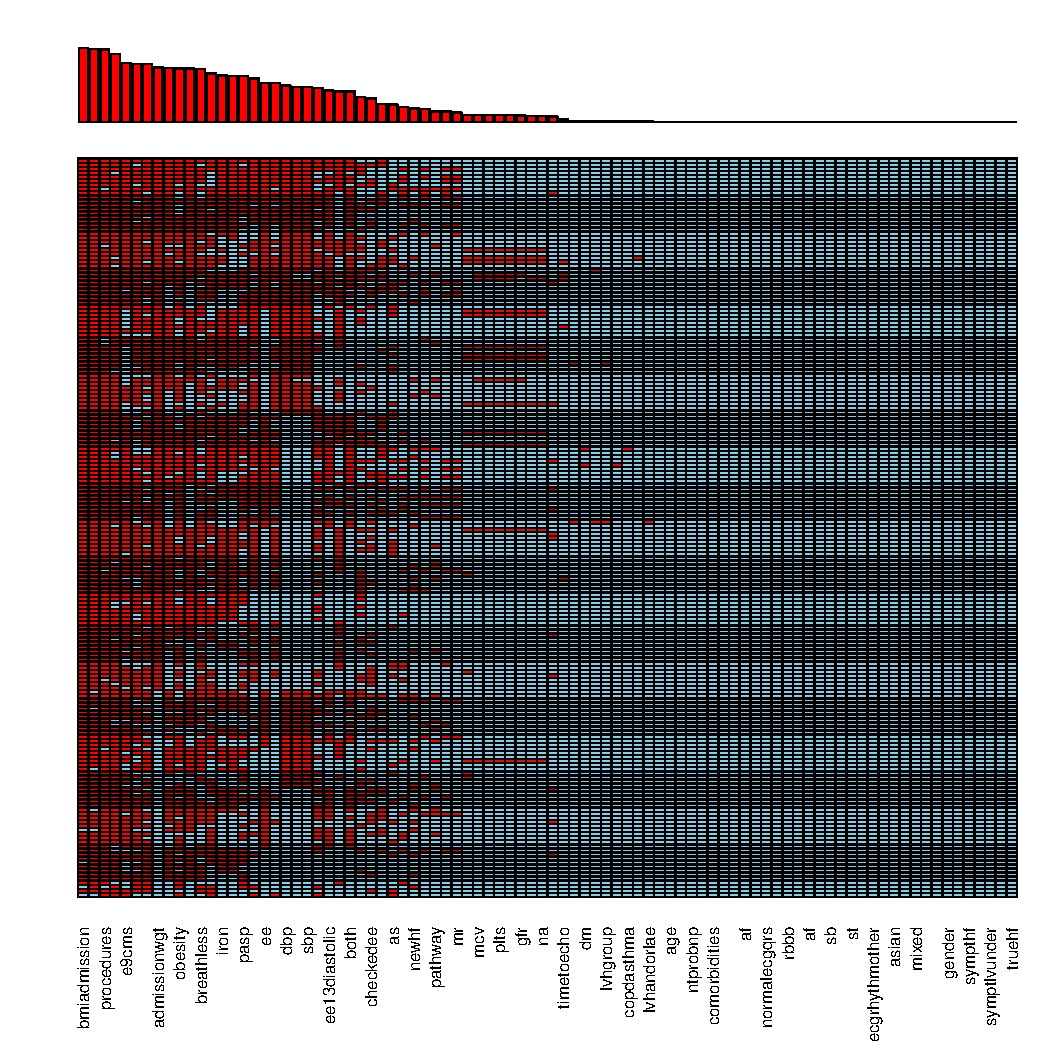
\includegraphics[width=1.1\textwidth]{doc/thesis/images/HFmrEF_miss_dist.pdf}
    \caption[Missing values in HFmrEF data set]{\textit{Missing values in HFmrEF data set. Top:  the amount of missing values in each variable sorted in ascending order. Bottom: plot of the combinations of missing (red) and non-missing (green) values in the HFmrEF data set.}}
    \label{fig:HFmrEF_missing}
\end{figure}

\newpage
\begin{figure}[h!]
    \centering
    % Created by tikzDevice version 0.11 on 2018-05-09 09:58:30
% !TEX encoding = UTF-8 Unicode
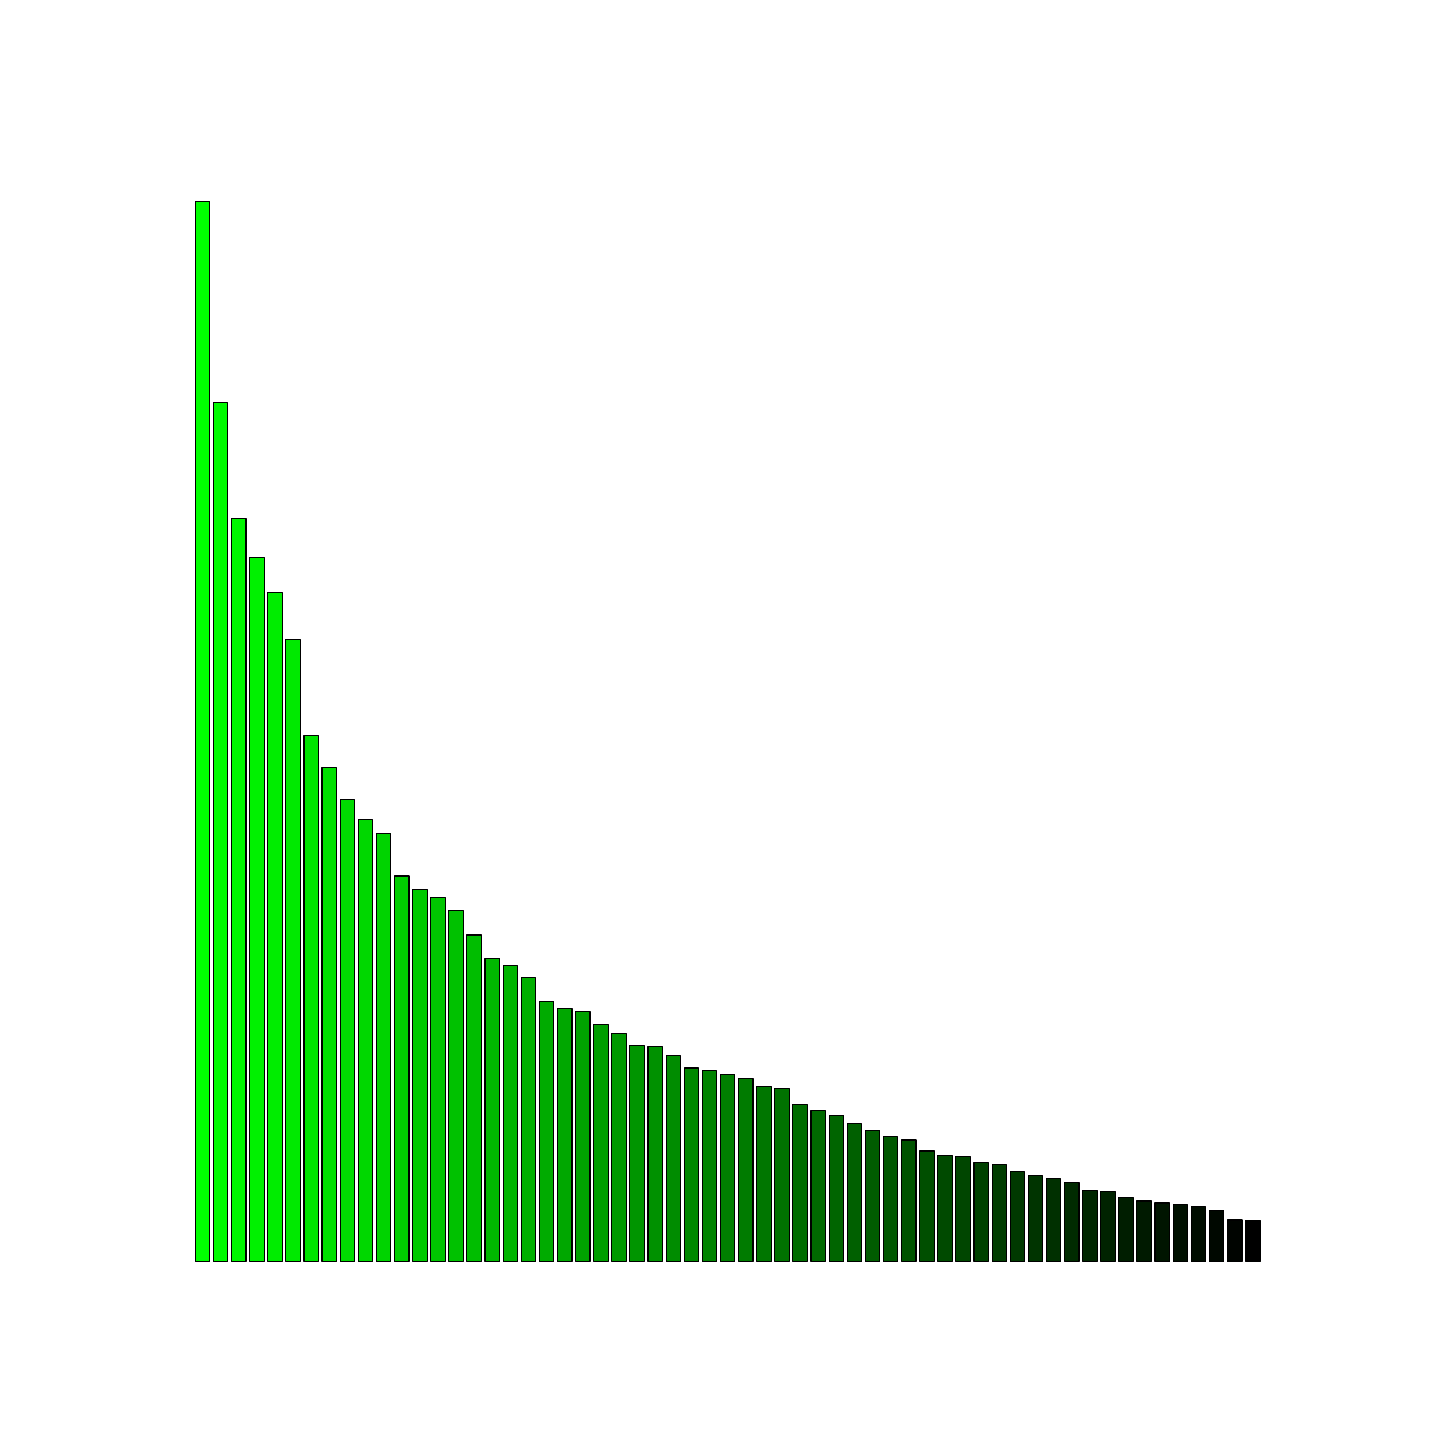
\begin{tikzpicture}[x=1pt,y=1pt]
\definecolor{fillColor}{RGB}{255,255,255}
\path[use as bounding box,fill=fillColor,fill opacity=0.00] (0,0) rectangle (505.89,505.89);
\begin{scope}
\path[clip] ( 48.00, 60.00) rectangle (457.89,457.89);
\definecolor{drawColor}{RGB}{0,0,0}
\definecolor{fillColor}{RGB}{0,255,0}

\path[draw=drawColor,line width= 0.4pt,line join=round,line cap=round,fill=fillColor] ( 60.56, 60.00) rectangle ( 65.80,443.15);
\definecolor{fillColor}{RGB}{0,250,0}

\path[draw=drawColor,line width= 0.4pt,line join=round,line cap=round,fill=fillColor] ( 67.11, 60.00) rectangle ( 72.34,370.44);
\definecolor{fillColor}{RGB}{0,246,0}

\path[draw=drawColor,line width= 0.4pt,line join=round,line cap=round,fill=fillColor] ( 73.65, 60.00) rectangle ( 78.89,328.47);
\definecolor{fillColor}{RGB}{0,241,0}

\path[draw=drawColor,line width= 0.4pt,line join=round,line cap=round,fill=fillColor] ( 80.19, 60.00) rectangle ( 85.43,314.38);
\definecolor{fillColor}{RGB}{0,237,0}

\path[draw=drawColor,line width= 0.4pt,line join=round,line cap=round,fill=fillColor] ( 86.74, 60.00) rectangle ( 91.97,301.74);
\definecolor{fillColor}{RGB}{0,233,0}

\path[draw=drawColor,line width= 0.4pt,line join=round,line cap=round,fill=fillColor] ( 93.28, 60.00) rectangle ( 98.52,284.82);
\definecolor{fillColor}{RGB}{0,228,0}

\path[draw=drawColor,line width= 0.4pt,line join=round,line cap=round,fill=fillColor] ( 99.83, 60.00) rectangle (105.06,250.18);
\definecolor{fillColor}{RGB}{0,224,0}

\path[draw=drawColor,line width= 0.4pt,line join=round,line cap=round,fill=fillColor] (106.37, 60.00) rectangle (111.60,238.52);
\definecolor{fillColor}{RGB}{0,219,0}

\path[draw=drawColor,line width= 0.4pt,line join=round,line cap=round,fill=fillColor] (112.91, 60.00) rectangle (118.15,226.92);
\definecolor{fillColor}{RGB}{0,215,0}

\path[draw=drawColor,line width= 0.4pt,line join=round,line cap=round,fill=fillColor] (119.46, 60.00) rectangle (124.69,219.61);
\definecolor{fillColor}{RGB}{0,211,0}

\path[draw=drawColor,line width= 0.4pt,line join=round,line cap=round,fill=fillColor] (126.00, 60.00) rectangle (131.23,214.78);
\definecolor{fillColor}{RGB}{0,206,0}

\path[draw=drawColor,line width= 0.4pt,line join=round,line cap=round,fill=fillColor] (132.54, 60.00) rectangle (137.78,199.34);
\definecolor{fillColor}{RGB}{0,202,0}

\path[draw=drawColor,line width= 0.4pt,line join=round,line cap=round,fill=fillColor] (139.09, 60.00) rectangle (144.32,194.32);
\definecolor{fillColor}{RGB}{0,197,0}

\path[draw=drawColor,line width= 0.4pt,line join=round,line cap=round,fill=fillColor] (145.63, 60.00) rectangle (150.87,191.69);
\definecolor{fillColor}{RGB}{0,193,0}

\path[draw=drawColor,line width= 0.4pt,line join=round,line cap=round,fill=fillColor] (152.17, 60.00) rectangle (157.41,186.94);
\definecolor{fillColor}{RGB}{0,189,0}

\path[draw=drawColor,line width= 0.4pt,line join=round,line cap=round,fill=fillColor] (158.72, 60.00) rectangle (163.95,178.03);
\definecolor{fillColor}{RGB}{0,184,0}

\path[draw=drawColor,line width= 0.4pt,line join=round,line cap=round,fill=fillColor] (165.26, 60.00) rectangle (170.50,169.60);
\definecolor{fillColor}{RGB}{0,180,0}

\path[draw=drawColor,line width= 0.4pt,line join=round,line cap=round,fill=fillColor] (171.80, 60.00) rectangle (177.04,166.92);
\definecolor{fillColor}{RGB}{0,175,0}

\path[draw=drawColor,line width= 0.4pt,line join=round,line cap=round,fill=fillColor] (178.35, 60.00) rectangle (183.58,162.63);
\definecolor{fillColor}{RGB}{0,171,0}

\path[draw=drawColor,line width= 0.4pt,line join=round,line cap=round,fill=fillColor] (184.89, 60.00) rectangle (190.13,154.09);
\definecolor{fillColor}{RGB}{0,167,0}

\path[draw=drawColor,line width= 0.4pt,line join=round,line cap=round,fill=fillColor] (191.44, 60.00) rectangle (196.67,151.41);
\definecolor{fillColor}{RGB}{0,162,0}

\path[draw=drawColor,line width= 0.4pt,line join=round,line cap=round,fill=fillColor] (197.98, 60.00) rectangle (203.21,150.50);
\definecolor{fillColor}{RGB}{0,158,0}

\path[draw=drawColor,line width= 0.4pt,line join=round,line cap=round,fill=fillColor] (204.52, 60.00) rectangle (209.76,145.67);
\definecolor{fillColor}{RGB}{0,153,0}

\path[draw=drawColor,line width= 0.4pt,line join=round,line cap=round,fill=fillColor] (211.07, 60.00) rectangle (216.30,142.52);
\definecolor{fillColor}{RGB}{0,149,0}

\path[draw=drawColor,line width= 0.4pt,line join=round,line cap=round,fill=fillColor] (217.61, 60.00) rectangle (222.84,138.07);
\definecolor{fillColor}{RGB}{0,145,0}

\path[draw=drawColor,line width= 0.4pt,line join=round,line cap=round,fill=fillColor] (224.15, 60.00) rectangle (229.39,137.58);
\definecolor{fillColor}{RGB}{0,140,0}

\path[draw=drawColor,line width= 0.4pt,line join=round,line cap=round,fill=fillColor] (230.70, 60.00) rectangle (235.93,134.45);
\definecolor{fillColor}{RGB}{0,136,0}

\path[draw=drawColor,line width= 0.4pt,line join=round,line cap=round,fill=fillColor] (237.24, 60.00) rectangle (242.48,129.97);
\definecolor{fillColor}{RGB}{0,131,0}

\path[draw=drawColor,line width= 0.4pt,line join=round,line cap=round,fill=fillColor] (243.78, 60.00) rectangle (249.02,128.91);
\definecolor{fillColor}{RGB}{0,127,0}

\path[draw=drawColor,line width= 0.4pt,line join=round,line cap=round,fill=fillColor] (250.33, 60.00) rectangle (255.56,127.68);
\definecolor{fillColor}{RGB}{0,123,0}

\path[draw=drawColor,line width= 0.4pt,line join=round,line cap=round,fill=fillColor] (256.87, 60.00) rectangle (262.11,126.21);
\definecolor{fillColor}{RGB}{0,118,0}

\path[draw=drawColor,line width= 0.4pt,line join=round,line cap=round,fill=fillColor] (263.41, 60.00) rectangle (268.65,123.34);
\definecolor{fillColor}{RGB}{0,114,0}

\path[draw=drawColor,line width= 0.4pt,line join=round,line cap=round,fill=fillColor] (269.96, 60.00) rectangle (275.19,122.47);
\definecolor{fillColor}{RGB}{0,109,0}

\path[draw=drawColor,line width= 0.4pt,line join=round,line cap=round,fill=fillColor] (276.50, 60.00) rectangle (281.74,116.77);
\definecolor{fillColor}{RGB}{0,105,0}

\path[draw=drawColor,line width= 0.4pt,line join=round,line cap=round,fill=fillColor] (283.05, 60.00) rectangle (288.28,114.47);
\definecolor{fillColor}{RGB}{0,101,0}

\path[draw=drawColor,line width= 0.4pt,line join=round,line cap=round,fill=fillColor] (289.59, 60.00) rectangle (294.82,112.87);
\definecolor{fillColor}{RGB}{0,96,0}

\path[draw=drawColor,line width= 0.4pt,line join=round,line cap=round,fill=fillColor] (296.13, 60.00) rectangle (301.37,109.91);
\definecolor{fillColor}{RGB}{0,92,0}

\path[draw=drawColor,line width= 0.4pt,line join=round,line cap=round,fill=fillColor] (302.68, 60.00) rectangle (307.91,107.53);
\definecolor{fillColor}{RGB}{0,87,0}

\path[draw=drawColor,line width= 0.4pt,line join=round,line cap=round,fill=fillColor] (309.22, 60.00) rectangle (314.45,105.12);
\definecolor{fillColor}{RGB}{0,83,0}

\path[draw=drawColor,line width= 0.4pt,line join=round,line cap=round,fill=fillColor] (315.76, 60.00) rectangle (321.00,103.94);
\definecolor{fillColor}{RGB}{0,79,0}

\path[draw=drawColor,line width= 0.4pt,line join=round,line cap=round,fill=fillColor] (322.31, 60.00) rectangle (327.54, 99.96);
\definecolor{fillColor}{RGB}{0,74,0}

\path[draw=drawColor,line width= 0.4pt,line join=round,line cap=round,fill=fillColor] (328.85, 60.00) rectangle (334.09, 98.48);
\definecolor{fillColor}{RGB}{0,70,0}

\path[draw=drawColor,line width= 0.4pt,line join=round,line cap=round,fill=fillColor] (335.39, 60.00) rectangle (340.63, 97.84);
\definecolor{fillColor}{RGB}{0,65,0}

\path[draw=drawColor,line width= 0.4pt,line join=round,line cap=round,fill=fillColor] (341.94, 60.00) rectangle (347.17, 95.79);
\definecolor{fillColor}{RGB}{0,61,0}

\path[draw=drawColor,line width= 0.4pt,line join=round,line cap=round,fill=fillColor] (348.48, 60.00) rectangle (353.72, 95.01);
\definecolor{fillColor}{RGB}{0,57,0}

\path[draw=drawColor,line width= 0.4pt,line join=round,line cap=round,fill=fillColor] (355.02, 60.00) rectangle (360.26, 92.41);
\definecolor{fillColor}{RGB}{0,52,0}

\path[draw=drawColor,line width= 0.4pt,line join=round,line cap=round,fill=fillColor] (361.57, 60.00) rectangle (366.80, 91.07);
\definecolor{fillColor}{RGB}{0,48,0}

\path[draw=drawColor,line width= 0.4pt,line join=round,line cap=round,fill=fillColor] (368.11, 60.00) rectangle (373.35, 89.97);
\definecolor{fillColor}{RGB}{0,43,0}

\path[draw=drawColor,line width= 0.4pt,line join=round,line cap=round,fill=fillColor] (374.66, 60.00) rectangle (379.89, 88.72);
\definecolor{fillColor}{RGB}{0,39,0}

\path[draw=drawColor,line width= 0.4pt,line join=round,line cap=round,fill=fillColor] (381.20, 60.00) rectangle (386.43, 85.69);
\definecolor{fillColor}{RGB}{0,35,0}

\path[draw=drawColor,line width= 0.4pt,line join=round,line cap=round,fill=fillColor] (387.74, 60.00) rectangle (392.98, 85.39);
\definecolor{fillColor}{RGB}{0,30,0}

\path[draw=drawColor,line width= 0.4pt,line join=round,line cap=round,fill=fillColor] (394.29, 60.00) rectangle (399.52, 83.21);
\definecolor{fillColor}{RGB}{0,26,0}

\path[draw=drawColor,line width= 0.4pt,line join=round,line cap=round,fill=fillColor] (400.83, 60.00) rectangle (406.06, 81.89);
\definecolor{fillColor}{RGB}{0,21,0}

\path[draw=drawColor,line width= 0.4pt,line join=round,line cap=round,fill=fillColor] (407.37, 60.00) rectangle (412.61, 81.17);
\definecolor{fillColor}{RGB}{0,17,0}

\path[draw=drawColor,line width= 0.4pt,line join=round,line cap=round,fill=fillColor] (413.92, 60.00) rectangle (419.15, 80.50);
\definecolor{fillColor}{RGB}{0,13,0}

\path[draw=drawColor,line width= 0.4pt,line join=round,line cap=round,fill=fillColor] (420.46, 60.00) rectangle (425.70, 79.78);
\definecolor{fillColor}{RGB}{0,8,0}

\path[draw=drawColor,line width= 0.4pt,line join=round,line cap=round,fill=fillColor] (427.00, 60.00) rectangle (432.24, 78.63);
\definecolor{fillColor}{RGB}{0,4,0}

\path[draw=drawColor,line width= 0.4pt,line join=round,line cap=round,fill=fillColor] (433.55, 60.00) rectangle (438.78, 75.04);
\definecolor{fillColor}{RGB}{0,0,0}

\path[draw=drawColor,line width= 0.4pt,line join=round,line cap=round,fill=fillColor] (440.09, 60.00) rectangle (445.33, 74.74);
\end{scope}
\end{tikzpicture}

\end{figure}


\chapter{Source Code}
\label{chap:souce_code}

\noindent The following appendix presents all the relevant \texttt{R}-code used in this thesis. We have organized the chapter in accordance with the various steps in the machine learning procedure adopted in this thesis, see figure (\ref{fig:ML_proc_thesis}). We have tried to comment as much of the source code in order to ensure that an eventual re-examination of the results can be as easy and smooth as possible. Inquires about the code can be forwarded to the author on request.

\section{Helper Functions, \texttt{\_helper\_func.R}}
\label{sec:helper_func}

\lstinputlisting[language=R]{../../data/data_sets/source/_helper_func.R}

\section{Load Data and Labeling, \texttt{r\_data\_sets.R}}
\label{sec:load_data}

\lstinputlisting[language=R]{../../data/data_sets/raw_data/r_data_sets.R}

\section{Data Description, \texttt{desc\_data.R}}
\label{sec:app_desc_stat}

\lstinputlisting[language=R]{../../data/data_sets/source/desc_data.R}

\section{Imputation, \texttt{imputation.R}}
\label{sec:app_impu}

\lstinputlisting[language=R]{../../data/data_sets/source/imputation.R}

\section{Dimensional Reduction, \texttt{dim\_reduc.R}}
\label{sec:dim_red}


\end{document}